\documentclass[a4paper,10pt]{jsarticle}
\usepackage{memo1}
% - - - - - - - - - 以下,個別編集箇所 - - - - - - - - - 
%タイトル
%左上のヘッダーにも表示される
\title{非平衡多体理論}
%署名
\affiliation{中国科学院大学 Kavli理論科学研究所}
\author{藤本純治}
%メールアドレス
\email{junji@ucas.ac.cn}
%作成・更新日とバージョンを書けばいいと思うよ
\date{2020-04-05}
%
\graphicspath{{./figure/}}
% - - - - - - - - - 以上,個別編集箇所 - - - - - - - - - 
\usepackage{memo2}
\usepackage{macro}
%\usepackage{diff}
%
\newcommand{\mH}{\mathrm{H}}
%
% 以下2つは参考文献の書式を指定する.bibtex を使わない場合はコメントアウト
%\bibliographystyle{apsrev4-1}
%\usepackage[numbers]{natbib}
%
\begin{document}
%
\maketitle

% abstract is here.
\begin{abstract}
このメモは主に,H.~J.~W.~HaugとA.-P.~Jauhoによる著書"\textit{Quantum Kinetics in Transport and Optics of Semiconductors}"のPart IIに従う.
まず前準備として,径路順序Green関数を定義し,それがcausal, greater, lesser, antitime-ordered Green関数に分解できることを見る.
次に,径路順序Green関数の摂動展開について調べる.
それから,径路順序Green関数の積を実時間の各種Green関数の積に書き換えるときに有用なLangreth則を紹介する.
以上の準備ののち,lesser Green関数の時間発展を記す方程式である量子運動方程式をKadanoffとBaymの方法に基づいて議論する.
\end{abstract}

%-%-%-%-%-%-%-%-%-%--%-%-%-%-%-%-%-%-%-%
\section{径路順序Green関数}
%-%-%-%-%-%-%-%-%-%--%-%-%-%-%-%-%-%-%-%
%-%-%-%-%-%-%-%-%-%-
\subsection{総説}
%-%-%-%-%-%-%-%-%-%-
非平衡問題は以下のように定式化される.
以下のハミルトニアンのもとで時間発展する系を考える.
\begin{align}
H
	& = h + H' (t)
.\end{align}
ここでハミルトニアンにおいて時間に依存しない部分$h$を2つの部分に分ける:$h = H_0 + H_i$,ただし$H_0$は(対角化でき,それゆえにWickの定理が適用できるという意味で)``シンプル''であり,$H_i$は(問題の多体的側面を含んでおり,それゆえに特別な取り扱いが必要であるという意味で)``複雑''であるとする.
さらに仮定として,非平衡部分は$t < t_0$においては消えるとする.

適切な時点で$t_0 \to - \infty$と置き換えることがしばしばある.
この手続きは問題の取り扱いを単純化し,非平衡理論の構造を可能な限り簡潔に示すことができるので,まず初めはこの極限を採用する.
しかし,そのような極限をとってしまうと過渡現象(transient phenomena)を取り扱うことが不可能になってしまう.
過渡現象は我々が述べたい中心的話題の一つなので,また必要なときにこの点に戻ってくることにする.
(このメモでは戻ってきません.)

摂動を加える前では,系は熱平衡の密度行列
\begin{align}
\rho (h)
	& = \frac{ \exp( - \beta h) }{ \mathrm{Tr}[ \exp(- \beta h) ] }
\end{align}
によって記述されている.
$\beta = 1 / \kB T$は逆温度である.
遂行すべきことは,与えられた観測量の期待値を計算することである.
その観測量に関連づけられた量子力学的な演算子を$O$とすると,時刻$t > t_0$においては,その期待値は
\begin{align}
\langle O (t) \rangle
	& = \mathrm{Tr} [ \rho (h) O_{H} (t) ]
\label{def:O}
\end{align}
と書ける.
下付き添字$H$は,Heisenberg描像で,その時間依存性は全ハミルトニアン$H$によって支配されていることを意味している.
定義~(\ref{def:O})は,容易に2時刻(あるいはそれ以上)の量(たとえばGreen関数や相関関数)に一般化することができる.

ここで,式~(\ref{def:O})において,何らかの時間依存した密度行列ではなく,熱平衡密度行列を用いたことを記しておく.
これは,物理的には,$h$に含まれている熱力学的な自由度は,$H'(t)$に含まれる速い振動に即座に追従しないことを意味している.
この他に選び方があってもよいが,それに伴う困難~\footnote{たとえば,文献~\cite{Mahan}のp.214-216を参照.}を避けるため,ここではこの選び方を採用する.
潜在的にとても見込みのある代替的方法は,期待値に含まれる熱平衡密度行列を,ある適切な一般化したものに置き換えることで構成され,それはHershfieldなどによって指摘され~\cite{Hershfield},近年いくつかの文献~\cite{Bokes,Coleman,Doyon,Han}において精巧化された.
この方法の可能性についても,半導体微細構造における時間依存輸送について書かれた13章で述べる.

%-%-%-%-%-%-%-%-%-%-
\subsection{2つの変換}
%-%-%-%-%-%-%-%-%-%-
式~(\ref{def:O})を攻略する一般的な戦略は,熱平衡の場合に似ている.
すなわち,$O_H (t)$の``望みが薄そうなほどに複雑な"時間依存性を,より簡単な$O_{H_0}$の時間依存の形へと変換させることである.
消去すべき演算子は2つある;時間依存する外的摂動$H' (t)$と``複雑な''相互作用項$H_i$である.
したがって,熱平衡の場合よりも込み入った変換を行うことが予想される.
しかしながら,適当に一般化することにともなって,非平衡と熱平衡の定式化を構造的に等価に行うことができると示せる.

最初に,$O_H$の時間依存性を$O_h$の時間依存性に書き換える.
これは,次の関係式を用いて行う.
\begin{align}
O_H (t)
	& = v_h^{\dagger} (t, t_0) O_h (t) v_h (t, t_0)
\label{eq:O_H}
,\end{align}
ここで
\begin{align}
v_h (t, t_0)
	& = \mathrm{T} \left\{ \exp \left[ - \zi \int_{t_0}^{t} \dd{t'} H'_h (t') \right] \right\}
,\end{align}
また$H'_h (t)$は$H' (t)$の相互作用表示で,
\begin{align}
H'_h (t)
	& = e^{\zi h (t - t_0)} H' (t) e^{- \zi h (t - t_0)}
\end{align}
で与えられ,$\mathrm{T}$は遅い時刻を左から並べていく時間順序演算子を表す.

ここで径路順序量を導入しよう.
表式~(\ref{eq:O_H})はまた別の,しかし等価な表式に書き換えることができる.
\begin{align}
O_H (t)
	& = \mathrm{T}_{C_t} \left\{ \exp \left[ - \zi \int_{C_t} \dd{\tau} H'_h (\tau) \right] O_h (t) \right\}
\label{eq:O_H_Ct}
,\end{align}
ただし,径路$C_t$は図~\ref{fig:4.1}に示す.
%%%%%%%%%%%%%%%%%%%%%%%%%%%%%%%%%%%%%%%%%%
\begin{figure}[thbp]
\centering
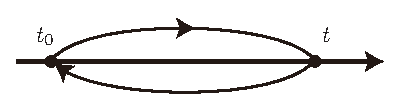
\includegraphics[width=0.5\linewidth]{4.1.eps}
\caption{\label{fig:4.1}径路$C_t$.}
\end{figure}
%%%%%%%%%%%%%%%%%%%%%%%%%%%%%%%%%%%%%%%%%%
以下では,複素径路上の時刻を表す変数をギリシャ文字で表記し,実時刻を表す変数に対してはローマ文字を用いるようにする.
経路$C_t$は,$t_0$から$t$に向けて実軸上を走り,もう一度$t$から$t_0$に戻る.
(あるいは,実軸の少しだけ上を走る;$H' (t)$が解析的に連続であるならば何ら問題は起こらない.)
経路順序演算子$T_{C_t}$の意味は,次のようになる.
$t_1$と$t_2$が$C_t$上の2つの時刻を表すとして,経路上で$t_2$が$t_1$に対して後に現れるならば,$T_{C_t} \{H'_h (t_1) H'_h (t_2)\} = H'_h (t_2) H'_h (t_1)$のように,後ろの時刻を左に並べかえる演算を表す.
次の計算で経路上に定義された関数の性質を示す.

%-%-%-%-%-%-%-%-%-%-%-
\textbf{式~(\ref{eq:O_H})と式~(\ref{eq:O_H_Ct})が等しいことを示す}\\
%-%-%-%-%-%-%-%-%-%-%-
経路上で定義された関数について理解を深めるために,ここで式~(\ref{eq:O_H})と式~(\ref{eq:O_H_Ct})が厳密に等しいことを示そう.
まず,式~(\ref{eq:O_H_Ct})に対して$\exp$を展開する.
\begin{align}
\mathrm{T}_{C_t} \left\{ \exp \left[ - \zi \int_{C_t} \dd{\tau} H'_h (\tau) \right] O_h (t) \right\}
	& = \sum_{n = 0}^{\infty} \frac{(-\zi)^n}{n!} \int_{C_t} \dd{\tau_1} \cdots \int_{C_t} \dd{\tau_n}
		\mathrm{T}_{C_t} \left[
			H'_h (\tau_1) \cdots H'_h (\tau_n) O_h (t)
		\right]
\label{eq:4.8}
.\end{align}
ここで,経路$C_t$を2つに分ける:
\begin{align}
\int_{C_t}
	& = \int_{\rightarrow} + \int_{\leftarrow}
,\end{align}
ただし$\int_{\rightarrow}$は$t_0$から$t$へ向かい,$\int_{\leftarrow}$は$t$から$t_0$に戻ることを表している.
よって,式~(\ref{eq:4.8})の$n$次の項は$2^n$個の項に分けられるが,そのうちの1つについて考えてみると,
\begin{align}
& \int_{\rightarrow} \dd{\tau_1} \int_{\rightarrow} \dd{\tau_2} \int_{\leftarrow} \dd{\tau_3} \cdots \int_{\leftarrow} \dd{\tau_n}
	\mathrm{T}_{C_t} \left[ H'_h (\tau_1) \cdots H'_h (\tau_n) O_h (t) \right]
\notag \\ & \hspace{1em}
	= \int_{\leftarrow} \dd{\tau_3} \cdots \int_{\leftarrow} \dd{\tau_n} \mathrm{T}_{\leftarrow} \left[ H'_h (\tau_3) \cdots H'_h (\tau_n) \right]
	O_h (t)
	\int_{\rightarrow} \dd{\tau_1} \int_{\rightarrow} \dd{\tau_2} \mathrm{T}_{\rightarrow} \left[ H'_h (\tau_1) H'_h (\tau_2) \right]
.\end{align}
$2^n$個の項のうち,$m \,(m = 0, \cdots, n)$個の$\int_{\rightarrow}$を含み,$n-m$個の$\int_{\leftarrow}$を含む項は$n! / [m! (n-m)!]$つあり,それらは全て等しく寄与する.
よって,
\begin{align}
& \int_{C_t} \dd{\tau_1} \cdots \int_{C_t} \dd{\tau_n} \mathrm{T}_{C_t} \left[ H'_h (\tau_1) \cdots H'_h (\tau_n) O_h (t) \right]
\notag \\ & \hspace{1em}
	= \sum_{m = 0}^{n} \frac{n!}{m! (n-m)!}
	\int_{\leftarrow} \dd{\tau_{m+1}} \cdots \int_{\leftarrow} \dd{\tau_n} \mathrm{T}_{\leftarrow} \left[ H'_h (\tau_{m+1}) \cdots H'_h (\tau_n) \right]
	O_h (t)
\notag \\ & \hspace{4em} \times
	\int_{\rightarrow} \dd{\tau_1} \cdots \int_{\rightarrow} \dd{\tau_m} \mathrm{T}_{\rightarrow} \left[ H'_h (\tau_1) \cdots H'_h (\tau_m) \right]	
\label{eq:4.11}
\end{align}
と書ける.
$k = n - m$と変数を書き換え,Kroneckerのデルタを用いて$k + m = n$を保ちつつ$k$と$m$の和を$0$から$\infty$までとるように書き換える.
すると,式~(\label{eq:4.11})は,
\begin{align}
& \to \sum_{m, k = 0}^{\infty} \frac{n!}{m! k!} \delta_{n, k + m}
	\left\{
		\int_{\leftarrow} \dd{\tau_1} \cdots \int_{\leftarrow} \dd{\tau_k} \mathrm{T}_{\leftarrow} \left[ H'_h (\tau_1) \cdots H'_h (\tau_k) \right]
	\right\}
	O_h (t)
\notag \\ & \hspace{3em} \times
	\left\{
		\int_{\rightarrow} \dd{\tau_1} \cdots \int_{\rightarrow} \dd{\tau_m} \mathrm{T}_{\rightarrow} \left[ H'_h (\tau_1) \cdots H'_h (\tau_m) \right]
	\right\}
.\end{align}
さて,式~(\ref{eq:4.8})に戻ると,$n$の和は$\delta_{n, k+m}$のために簡単に実行でき,以下を得る.
\begin{align}
& \mathrm{T}_{C_t} \left\{ \exp \left[ - \zi \int_{C_t} \dd{\tau} H'_h (\tau) \right] O_h (t) \right\}
\notag \\ & \hspace{1em}
	= \sum_{k = 0}^{\infty} \frac{(-\zi)^k}{k!}
	\left\{
		\int_{\leftarrow} \dd{\tau_1} \cdots \int_{\leftarrow} \dd{\tau_k} \mathrm{T}_{\leftarrow} \left[ H'_h (\tau_1) \cdots H'_h (\tau_k) \right]
	\right\}
	O_h (t)
\notag \\ & \hspace{3em} \times
	\sum_{m = 0}^{\infty} \frac{(-\zi)^m}{m!}
	\left\{
		\int_{\rightarrow} \dd{\tau_1} \cdots \int_{\rightarrow} \dd{\tau_m} \mathrm{T}_{\rightarrow} \left[ H'_h (\tau_1) \cdots H'_h (\tau_m) \right]
	\right\}
.\end{align}
しかして,$O (t)$に左右から掛けられている因子を見比べると,それらがそれぞれ$v_h^{\dagger} (t_0, t)$と$v_h (t_0, t)$に等しいことが分かる.
以上で,式~(\ref{eq:O_H})と式~(\ref{eq:O_H_Ct})の等価性が示された.
■

経路順序演算子は,熱平衡理論と全く同じように非平衡理論を構築するのに強力な形式的道具である.

さて,経路順序Green関数(contour-ordered Green function)を定義しよう:
\begin{align}
G (x, x')
	& \equiv - \zi \langle \mathrm{T}_C [ \psi^{}_{\mH} (x) \psi^{\dagger}_{\mH} (x') ] \rangle
\label{def:G}
,\end{align}
ただし,経路$C$は$t_0$に始まり,同じ$t_0$で終わる図~\ref{fig:4.2}のような,実軸に沿って$t$と$t'$を一度だけ通るような経路を表す.
ここで,Part Iと同じように,$\psi_{\mH} (x)$はフェルミオンの場の演算子で,Heisenberg表示を表す.
また,以下では$x = (\br, t)$あるいは$x = (\br, \tau)$という簡略表記を用いる\footnote{原文では$1 = (\bm{x}_1, t_1$などと書かれているが,個人的にはあまり馴染みがないため,馴染みのある表記に書き換えた.}.
%%%%%%%%%%%%%%%%%%%%%%%%%%%%%%%%%%%%%%%%%%
\begin{figure}[thbp]
\centering
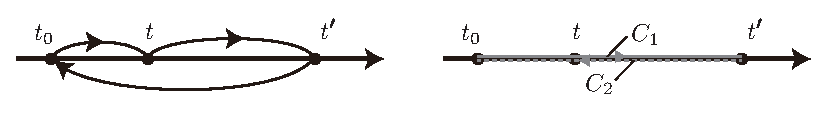
\includegraphics[width=\linewidth]{4.2.eps}
\caption{\label{fig:4.2}径路$C$.}
\end{figure}
%%%%%%%%%%%%%%%%%%%%%%%%%%%%%%%%%%%%%%%%%%

非平衡の理論において経路順序Green関数は,熱平衡の理論における因果Green関数に類似の役割を果たす.
すなわち,以下で見るように,Wickの定理に基づいた摂動展開を有している.
しかしながら,時刻ラベル$\tau$と$\tau'$は経路上の2つの分枝にあるため,それらがどの分枝にあるのかが問題になる.
$\tau$と$\tau'$は,図~\ref{fig:4.2}の経路の2つの分枝のどちらの分枝にもありうるので,4つの可能性がある.
ゆえに,式~(\ref{def:G})は,4つの異なる関数を内包する.
\begin{align}
G (x, x')
	& = \left\{
	\begin{array}{l l}
		G_{\mathrm{c}} (x, x')
	&	t, t' \in C_1
	\\	G^{>} (x, x')
	&	t \in C_2, t' \in C_1
	\\	G^{<} (x, x')
	&	t \in C_1, t' \in C_2
	\\	G_{\tilde{\mathrm{c}}} (x, x')
	&	t, t' \in C_2
	.\end{array}
	\right.
\end{align}
ここで,因果 (あるいは時間順序) Green関数$G_{\mathrm{c}}$を
\begin{align}
G_{\mathrm{c}} (x, x')
	& = - \zi \langle \mathrm{T} [ \psi^{}_{\mH} (x) \psi^{\dagger}_{\mH} (x') ] \rangle
\notag \\
	& = - \zi \theta (t - t') \langle \psi^{}_{\mH} (x) \psi^{\dagger}_{\mH} (x') \rangle
		+ \zi \theta (t' - t) \langle \psi^{\dagger}_{\mH} (x') \psi^{}_{\mH} (x) \rangle
\end{align}
のように,また``greater'' Green関数$G^{>}$を
\begin{align}
G^{>} (x, x')
	& = - \zi \langle \psi^{}_{\mH} (x) \psi^{\dagger}_{\mH} (x') \rangle
\end{align}
のように,そして``lesser'' Green関数$G^{<}$を
\begin{align}
G^{<} (x, x')
	& = + \zi \langle \psi^{\dagger}_{\mH} (x') \psi^{}_{\mH} (x) \rangle
\end{align}
のように,最後に反時間順序Green関数$G_{\tilde{\mathrm{c}}}$を
\begin{align}
G_{\tilde{\mathrm{c}}} (x, x')
	& = - \zi \langle \tilde{\mathrm{T}} [ \psi^{}_{\mH} (x) \psi^{\dagger}_{\mH} (x') ] \rangle
\notag \\
	& = - \zi \theta (t' - t) \langle \psi^{}_{\mH} (x) \psi^{\dagger}_{\mH} (x') \rangle
		+ \zi \theta (t - t') \langle \psi^{\dagger}_{\mH} (x') \psi^{}_{\mH} (x) \rangle
\end{align}
のように導入した.
$G_{\mathrm{c}} + G_{\tilde{\mathrm{c}}} = - \zi \langle \psi^{}_{\mH} (x) \psi^{\dagger}_{\mH} (x') \rangle + \zi \langle \psi^{\dagger}_{\mH} (x') \psi^{}_{\mH} (x) \rangle = G^{>} + G^{<}$なので,独立な関数は3つである.
この自由度の選び方には幾つかの流儀があり,幾つもの表記法が見られる.
我々の目的のために最も最適な関数は$G^{>}$と$G^{<}$(これらはしばしば「相関関数」という一般的な名前で書かれることもある)と,先進Green関数と遅延Green関数である.
先進Green関数は
\begin{align}
G^{\A} (x, x')
	& = \zi \theta (t' - t) \langle \{ \psi^{}_{\mH} (x), \psi^{\dagger}_{\mH} (x') \} \rangle
\notag \\
	& = - \theta (t' - t) \left[ G^{>} (x, x') - G^{<} (x, x') \right]
\end{align}
と遅延Green関数は
\begin{align}
G^{\R} (x, x')
	& = - \zi \theta (t - t') \langle \{ \psi^{}_{\mH} (x), \psi^{\dagger}_{\mH} (x') \} \rangle
\notag \\
	& = \theta (t - t') \left[ G^{>} (x, x') - G^{<} (x, x') \right]
\end{align}
で定義される.
ここで$\{A, B\} = A B + B A$は反交換関係を表す.
$G^{\R} (x, x') - G^{\A} (x, x') = G^{>} (x, x') - G^{<} (x, x')$が見てとれる.
後ろの章にて,$G^{>}, G^{<}, G^{\R}, G^{\A}$の物理的な解釈について詳細に議論する予定である({\color{red}どこ?}).

必要な関数の定義を終えて,本節の中心課題に戻るとする.
すなわち,経路順序Green関数~(\ref{def:G})をWickの定理を用いられる形に変形するということだ.
第一段階として,式~(\ref{eq:O_H_Ct})を導いた解析,つまり$H$依存性を$h$依存性に書き換えることをここでも繰り返す.
その結果は,\footnote{{\color{red} このあたりの計算が端折られている点が,あまり親切ではないと感じる点ではある.}}
\begin{align}
G (x, x')
	& = - \zi \langle \mathrm{T}_C [ S_{C}^{H} \psi^{}_{h} (x) \psi^{\dagger}_{h} (x') ] \rangle
\label{eq:G_H}
,\end{align}
ここで,$\psi^{(\dagger)}_{h} (x) = e^{\zi h (t - t_0)} \psi^{(\dagger)} (\br) e^{- \zi h (t - t_0)}$は$\psi^{(\dagger)} (\br)$の相互作用表示であり,
\begin{align}
S_{C}^{H}
	& = \exp \left[ - \zi \int_{C} \dd{\tau} H'_{h} (\tau) \right]
\end{align}
である.
ダイヤグラム的摂動理論が存在することを示すためには,さらにもう一段階の式変形が必要である.
$h = H_0 + H_i$のように$h$が2つの項を含んでいたこと,そしてWickの定理が$H_0$に対してのみ機能することを思い出せば,$h$依存性を$H_0$依存性に置き換えなければならないことになる.
また,密度行列にも$h$が含まれており,それゆえに,式~(\ref{eq:G_H})には,$\rho (h)$, $S_{C}^{H}$, $\psi^{}_h (x)$, $\psi^{\dagger}_h (x')$の合計で4箇所に$h$が含まれていることに留意する.

この式変形は,いくぶん退屈であるが躓くところはほとんどないはずなので,詳細は文献~\cite{RammerRMP}に譲り,最終結果を記すだけで十分だろう.~\footnote{{\color{red} このあたりの計算が端折られている点が,あまり親切ではないと感じる点ではある.}}
\begin{align}
G (x, x')
	& = - \zi \frac{ \mathrm{Tr} \left\{ \mathrm{T}_{C_v} [ S_{C_v}^i S'_{C} \psi^{}_{H_0} (x) \psi^{\dagger}_{H_0} (x') ] \right\} }%
		{ \mathrm{Tr} [ \rho_0 \mathrm{T}_{C_v} ( S_{C_v}^i S'_{C} ) ] }
\label{eq:G_H0}
,\end{align}
ここで,密度行列$\rho_0$は
\begin{align}
\rho_0
	& = \frac{\exp (- \beta H_0)}{\mathrm{Tr} [ \exp (- \beta H_0) ]}
\end{align}
で与えられ,
\begin{align}
S'_{C}
	& = \exp \left[ - \zi \int_{C} \dd{\tau} H'_{H_0} (\tau) \right]
\notag
, \\
S_{C_v}^i
	& = \exp \left[ - \zi \int_{C_v} \dd{\tau} H_{i, H_0} (\tau) \right]
\end{align}
であるが,$H'_{H_0}$と$H_{i, H_0}$は$H_0$による時間発展を表す;
\begin{align*}
H'_{H_0} (t)
	= e^{\zi H_0 (t - t_0)} H' e^{- \zi H_0 (t - t_0)}
, \qquad
H_{i, H_0} (t)
	= e^{\zi H_0 (t - t_0)} H_i e^{- \zi H_0 (t - t_0)}
.\end{align*}
また,経路$C$は図~\ref{fig:4.2}にて定義したものであり,経路$C_v$は図~\ref{fig:4.3}に示した.
%%%%%%%%%%%%%%%%%%%%%%%%%%%%%%%%%%%%%%%%%%
\begin{figure}[thbp]
\centering
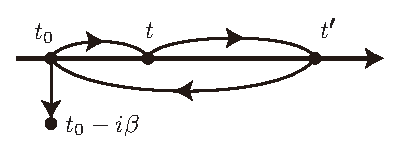
\includegraphics[width=0.5\linewidth]{4.3.eps}
\caption{\label{fig:4.3}径路$C_v$.}
\end{figure}
%%%%%%%%%%%%%%%%%%%%%%%%%%%%%%%%%%%%%%%%%%

式~(\ref{eq:G_H0})は,重要な結果であり,見た目の複雑さに関わらず,多くの魅力的な性質を有している.
まず第一に,厳密であるという点である.
次に,全ての時間依存性は,$H_0$によって記されているため,「解くことができる」.
特に,平方完成できる密度行列($\sim \exp( - \beta H_0)$)のために,Wickの定理を用いることが可能であり,そのためFeynmanダイヤグラムを非平衡系の問題に構成することができる.
ちょうど熱平衡系のときのように,分母が非連結のダイヤグラムからの寄与を打ち消してくれるのである.

以下のようにこの節の中心的な結果をまとめられる.
すなわち,熱平衡理論と非平衡理論は構造的に等価であり,それらの違いは,単に実時間における積分が経路上の積分に置き換えられただけである.


%-%-%-%-%-%-%-%-%-%-
\subsection{解析接続}
%-%-%-%-%-%-%-%-%-%-
















%\bibliography{name}

\begin{thebibliography}{99}
\bibitem{Mahan} G.~D.~Mahan, ``Many-Particle Physics'', 2nd edn. (Plenum, New York, 1990).
\bibitem{Hershfield} S. Hershfield: Phys. Rev. Lett. 70, 2135 (1993).
\bibitem{Bokes} P. Bokes, H. Mera, R. W. Godby: Phys. Rev. B 72 165425 (2005).
\bibitem{Coleman} P. Coleman, W. Mao: J. Phys. Cond. Matt. 16, L263 (2004).
\bibitem{Doyon} B. Doyon, N. Andrei: Phys. Rev. B 73, 245326 (2006).
\bibitem{Han} J. E. Han, Phys. Rev. B 73, 125319 (2006).
\bibitem{RammerRMP} J. Rammer, H. Smith: Rev. Mod. Phys. 58, 323 (1986).
\end{thebibliography}


\end{document}
